\section{Progettazione logica}

\subsection{Analisi delle ridondanze}
Le ridondanze corrispondono alla presenza di dati che possono essere derivati da altri. È quindi importante domandarsi se questa ridondanza crei solo confusione o velocizzi veramente le operazioni.

Nello schema concettuale possiamo individuare stato di occupazione che è deducibile dalla relazione sosta che presenta l'attributo data di arrivo e data di partenza.

Le operazioni coinvolte sono la numero 2 e la numero 6 che presentano una frequenza di 40 volte al giorno e 30-40 volte ogni giorno.

Si procede alla valutazione del costo totale in termini di accessi nel caso di ridondanza e di assenza di essa.

\begin{center}
    \begin{tabularx}{\textwidth}{|p{90mm}|X|}
        \hline
        \rowcolor{gray!30}
        \textbf{Operazione} & \textbf{Frequenza}\\
        \hline
        2. Controllo dei posti disponibili per una certa imbarcazione(Controllo delle dimensioni)& 40 volte al giorno\\
        \hline
        6. Arrivo di un'imbarcazione in uno dei marina & 30-40 volte al giorno\\
        \hline
    \end{tabularx}
\end{center}

Ci riferiremo per i nostri calcoli a dei volumi plausibili nella vita della base di dati. I moli non variano particolarmente di numero, le imbarcazioni vengono registrate al loro primo accesso e le soste aumentano ogni giorno. Mediamente un'imbarcazione sosta 2,7 volte in un molo.

\begin{center}
    \begin{tabularx}{\textwidth}{|X|X|X|}
        \hline
        \rowcolor{gray!30}
        \textbf{Concetto} & \textbf{Tipo} & \textbf{Volume}\\
        \hline
        Molo & ENTITÀ & 1600\\
        \hline
        Imbarcazione & ENTITÀ & 5000\\
        \hline
        Sosta & RELAZIONE & 13500\\ % Contando che ogni imbarcazione sosta in media due volte per molo.
        \hline
    \end{tabularx}
\end{center}

\paragraph{operazione 2}

\begin{center}
    \begin{minipage}{.48\linewidth}
        \begin{tabularx}{\linewidth}{|X|l|l|l|}
            \hline
            \rowcolor{gray!30}
            \multicolumn{4}{|c|}{\textbf{Con ridondanza}}\\
            \hline
            \rowcolor{gray!15}
            Concetto & Costrutto & Accessi & Tipo\\
            \hline
            Molo & E & 1600 & L\\
            \hline
        \end{tabularx}
    \end{minipage}
    \begin{minipage}{.48\linewidth}
        \begin{tabularx}{\linewidth}{|X|l|l|l|}
            \hline
            \rowcolor{gray!30}
            \multicolumn{4}{|c|}{\textbf{Senza ridondanza}}\\
            \hline
            \rowcolor{gray!15}
            Concetto & Costrutto & Accessi & Tipo\\
            \hline
            Sosta & R & 13500 & L\\
            \hline
            Molo & E & 1600 & L\\
            \hline
        \end{tabularx}
    \end{minipage}
\end{center}

\underline{Con ridondanza}
\begin{itemize}
    \item Totale accessi(Solo in lettura): $1600*40 = 64000$
\end{itemize}
\underline{Senza ridondanza}
\begin{itemize}
    \item Totale accessi(Solo in lettura): $1600*13500*40 = 864000000$ Giornalieri
\end{itemize}

\paragraph{operazione 6}

\begin{center}
    \begin{minipage}{.48\linewidth}
        \begin{tabularx}{\linewidth}{|X|l|l|l|}
            \hline
            \rowcolor{gray!30}
            \multicolumn{4}{|c|}{\textbf{Con ridondanza}}\\
            \hline
            \rowcolor{gray!15}
            Concetto & Costrutto & Accessi & Tipo\\
            \hline
            Imbarcazione & E & 1 & S\\
            \hline
            Sosta & R & 1 & S\\
            \hline
            Sosta & R & 1 & L\\
            \hline
            Molo & E & 1 & S\\
            \hline
        \end{tabularx}
    \end{minipage}
    \begin{minipage}{.48\linewidth}
        \begin{tabularx}{\linewidth}{|X|l|l|l|}
            \hline
            \rowcolor{gray!30}
            \multicolumn{4}{|c|}{\textbf{Senza ridondanza}}\\
            \hline
            \rowcolor{gray!15}
            Concetto & Costrutto & Accessi & Tipo\\
            \hline
            Imbarcazione & E & 1 & S\\
            \hline
            Sosta & R & 1 & S\\
            \hline
        \end{tabularx}
    \end{minipage}
\end{center}


Con ridondanza
\begin{itemize}
    \item Totale scritture: $40 + 40 + 40 = 120 \xrightarrow{*2} 240$ 
    \item Totale letture: $40$
    \item Totale accessi: $240+40 = 280$ Giornalieri
\end{itemize}
Senza ridondanza
\begin{itemize}
    \item Totale accessi(Solo in scrittura): $40+40 = 80 \xrightarrow{*2} 160 $ Giornalieri
\end{itemize}

\paragraph{In conclusione}
nell'\textbf{operazione 2} risulta meno costosa in termini di accessi l'operazione con ridondanza, nell'\textbf{operazione 6} invece risulta meno costosa in termini di accessi l'operazione senza ridondanza. Notando però che la prima delle due operazioni diventa spropositamene pesante senza ridondanza qui si sceglie di mantenere la ridondanza.

\subsubsection{altre ridondanze}

Le altre ridondanze sono:
\begin{enumerate}
    \item Quantità di moli in Marina è deducibile dalla relazione appartenenza e l'entità molo;
    \item Data prima arrivo in Cliente abituale è deducibile da Cliente possiede imbarcazione che sosta in un molo andando a vedere la data di arrivo più vecchia;
    \item Marina visitati in Cliente occasionale è deducibile da Cliente possiede imbarcazione che sosta in un molo andando a vedere quante soste hanno effettuato le sue imbarcazioni;
\end{enumerate}

In seguito all'analisi sugli accessi abbiamo stimato che tutte e tre risultino essere preferibili con ridondanza, relativamente ad eventuali operazioni di lettura e scrittura di questi valori. Pertanto si è deciso di mantenere le informazioni ridondanti.


\subsection{Eliminazione degli attributi multi-valore}

Contatto in Persona è multi-valore. Anche Orario apertura e orario chiusura in servizio sono multi-valore.

Dovrò quindi trasformarli in un'ER-relazione binaria. In particolare in servizio accorperò i due orari in orario di erogazione.

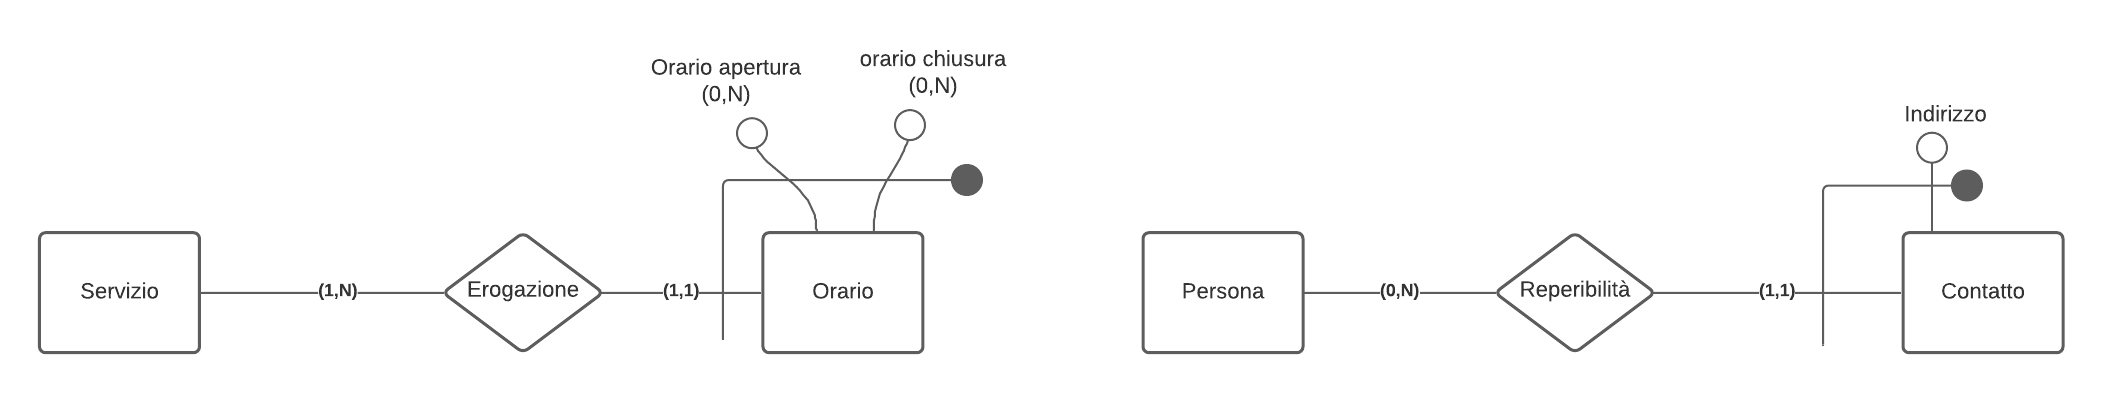
\includegraphics[width=\linewidth]{img/multi_valore.png}

\subsection{Eliminazione delle generalizzazioni}

Poichè i sistemi tradizionali per la gestione delle basi di dati non permettono di rappresentare in maniera diretta una generalizzazione, è necessario trasformare questo costrutto in Entità e relazioni:

\paragraph{Cliente}\mbox{}\\
Si accorpano Cliente abituale e cliente occasionale a Cliente. Dato che il numero di marina visitati e la data di primo arrivo sono attributi utili per entrambe le tipologie di cliente, vengono semplicemente aggiunti questi due attributi a Cliente. Inoltre aggiungiamo un booleano che definisce la differenza tra abituale e occasionale.
\paragraph{Persona}\mbox{}\\
La generalizzazione di persona, per evitare inutili valori NULL in un eventuale accorpamento viene trasformata nell'entità "Persona", questa entità conterrà tutti i dati relativi alla persona e avrà due entità deboli collegate ovvero Addetto e Cliente.

Persona avrà da 0 a 1 Cliente e da 0 a 1 Addetto. In Addetto e Cliente posizioneremo i dati relativi a queste due entità come da schema concettuale.

\subsection{Partizionamento/Accorpamento di entità e relazioni}

\subsection{Scelta degli identificatori primari}

\subsection{Traduzione verso il modello relazionale}
%Qui e dove definisco come devono essere scritti nel db le tabelle

\subsection{Schema concettuale ristrutturato - Schema logico}
%\includegraphics[width=\textwidth]{}

\subsection{vincoli di integrità referenziale}
